\documentclass[tikz]{standalone}

\begin{document}
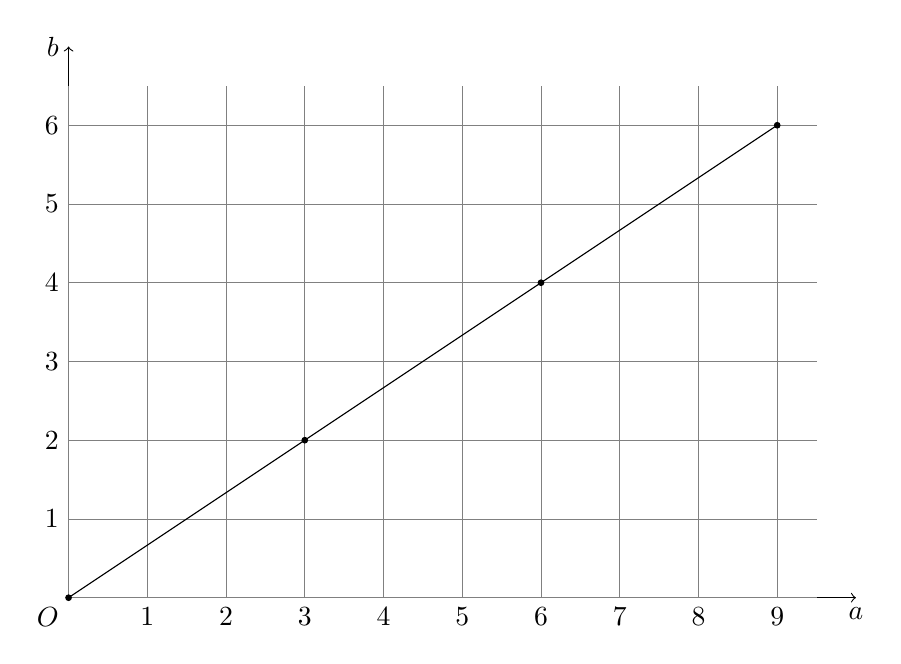
\begin{tikzpicture}[smooth]
    \draw[->] (0,0) node[anchor=north east]{$O$}--(10,0) node[below]{$a$};
    \draw[->] (0,0)--(0,7) node[anchor=east]{$b$};
    \draw[very thin,color=gray](0,0) grid (9.5, 6.5);
    \foreach \x in {1, 2, 3, 4, 5, 6, 7, 8, 9}
        \draw (\x, 0) node[anchor=north] {$\x$};
    \foreach \y in {1, 2, 3, 4, 5, 6}
        \draw (0, \y) node[anchor=east] {$\y$};

    \filldraw (0, 0) circle (1pt) -- (3, 2) circle (1pt) -- (6, 4) circle (1pt)
        -- (9, 6) circle (1pt);

\end{tikzpicture}
\end{document}
